\section{基本环境与图表算法}
%\sepframe[image={
\includegraphics[width=3.38cm]{./Figures/Logos/USTC_logo_blue.pdf}}]
% \sepframe 无插入 logo 的分隔页
\sepframe[image={
\includegraphics[width=3.38cm]{./Figures/Logos/USTC_logo_blue.pdf}}]



\begin{frame}[fragile,allowframebreaks]{常用基础环境}
%%%%%%%%%%%%%%%%%% frame %%%%%%%%%%%%%%%%%%
\begin{block}{Frame 环境}
	\texttt{frame} 用于在 Beamer 中新建\textbf{页面框架}，在框架中编写当前 \texttt{frame} 内容。可选参数常用：\texttt{[fragile, allowframebreaks, shrink, squeeze]}。
\end{block}
\begin{lstlisting}
\begin{frame}{Frame Title} % 内容页开始，\begin{frame}{} 则不显示 Frame Title
% 编写 Frame 内容
\end{frame} % 内容页结束
\end{lstlisting}

%%%%%%%%%%%%%%%%%% block %%%%%%%%%%%%%%%%%%
\begin{block}{Block 环境}
	这是 \texttt{block} 环境的示例文字。
\end{block}
\begin{lstlisting}
\begin{block}{Block Title} % \begin{block}{} 则不显示 Block Title
    这是 \texttt{block} 环境的示例文字。
\end{block}
\end{lstlisting}

%%%%%%%%%%%%%%%%%% information %%%%%%%%%%%%%%%%%%
\begin{information}[Information 环境]
这是 \texttt{Information} 环境的示例文字。
\end{information}
\begin{lstlisting}
\begin{information}[Information 环境] \begin{information} 则显示为 information
    这是 \texttt{Information} 环境的示例文字。
\end{information}
\end{lstlisting}
%%%%%%%%%%%%%%%%%% alertblock %%%%%%%%%%%%%%%%%%
\begin{alertblock}{AlertBlock 环境}
	这是 \texttt{Alertblock} 环境的示例文字。
\end{alertblock}
\begin{lstlisting}
\begin{alertblock}{AlertBlock Title} % \begin{alertblock}{} 则不显示 AlertBlock Title
    这是 \texttt{Alertblock} 环境的示例文字。
\end{alertblock}
\end{lstlisting}
	
	
%%%%%%%%%%%%%%%%%% exampleblock %%%%%%%%%%%%%%%%%%
\begin{exampleblock}{ExampleBlock 环境}
	这是 \texttt{ExampleBlock} 环境的示例文字。
\end{exampleblock}
\begin{lstlisting}
\begin{exampleblock}{ExampleBlock Title} % \begin{exampleblock}{} 则不显示 ExampleBlock Title
    这是 \texttt{ExampleBlock} 环境的示例文字。
\end{exampleblock}
\end{lstlisting}
\end{frame}


\begin{frame}[fragile,allowframebreaks]{列表环境}
	\begin{minipage}[t]{0.43\linewidth}
		\begin{itemize}
			\item 美食\begin{enumerate}
				\item 火锅
				\item 烧烤
			\end{enumerate}
			\item 运动\begin{itemize}
				\item 羽毛球
				\item 健身
			\end{itemize}
		\end{itemize}
\begin{lstlisting}
\begin{itemize}
    \item 美食\begin{enumerate}
        \item 火锅
        \item 烧烤
    \end{enumerate}
    \item 运动\begin{itemize}
        \item 羽毛球
        \item 健身
    \end{itemize}
\end{itemize}
\end{lstlisting}
	\end{minipage}\hspace*{1.5cm}
	\begin{minipage}[t]{0.43\linewidth}
		\begin{enumerate}
			\item 美食\begin{enumerate}
				\item 火锅
				\item 烧烤
			\end{enumerate}
			\item 运动\begin{itemize}
				\item 羽毛球
				\item 健身
			\end{itemize}
		\end{enumerate}
\begin{lstlisting}
\begin{enumerate}
    \item 美食\begin{enumerate}
        \item 火锅
        \item 烧烤
    \end{enumerate}
    \item 运动\begin{itemize}
        \item 羽毛球
        \item 健身
    \end{itemize}
\end{enumerate}
\end{lstlisting}
	\end{minipage}

\end{frame}

\begin{frame}[fragile,allowframebreaks]{图片}
\begin{block}{单张图}
	\begin{figure}[H]
		\centering
		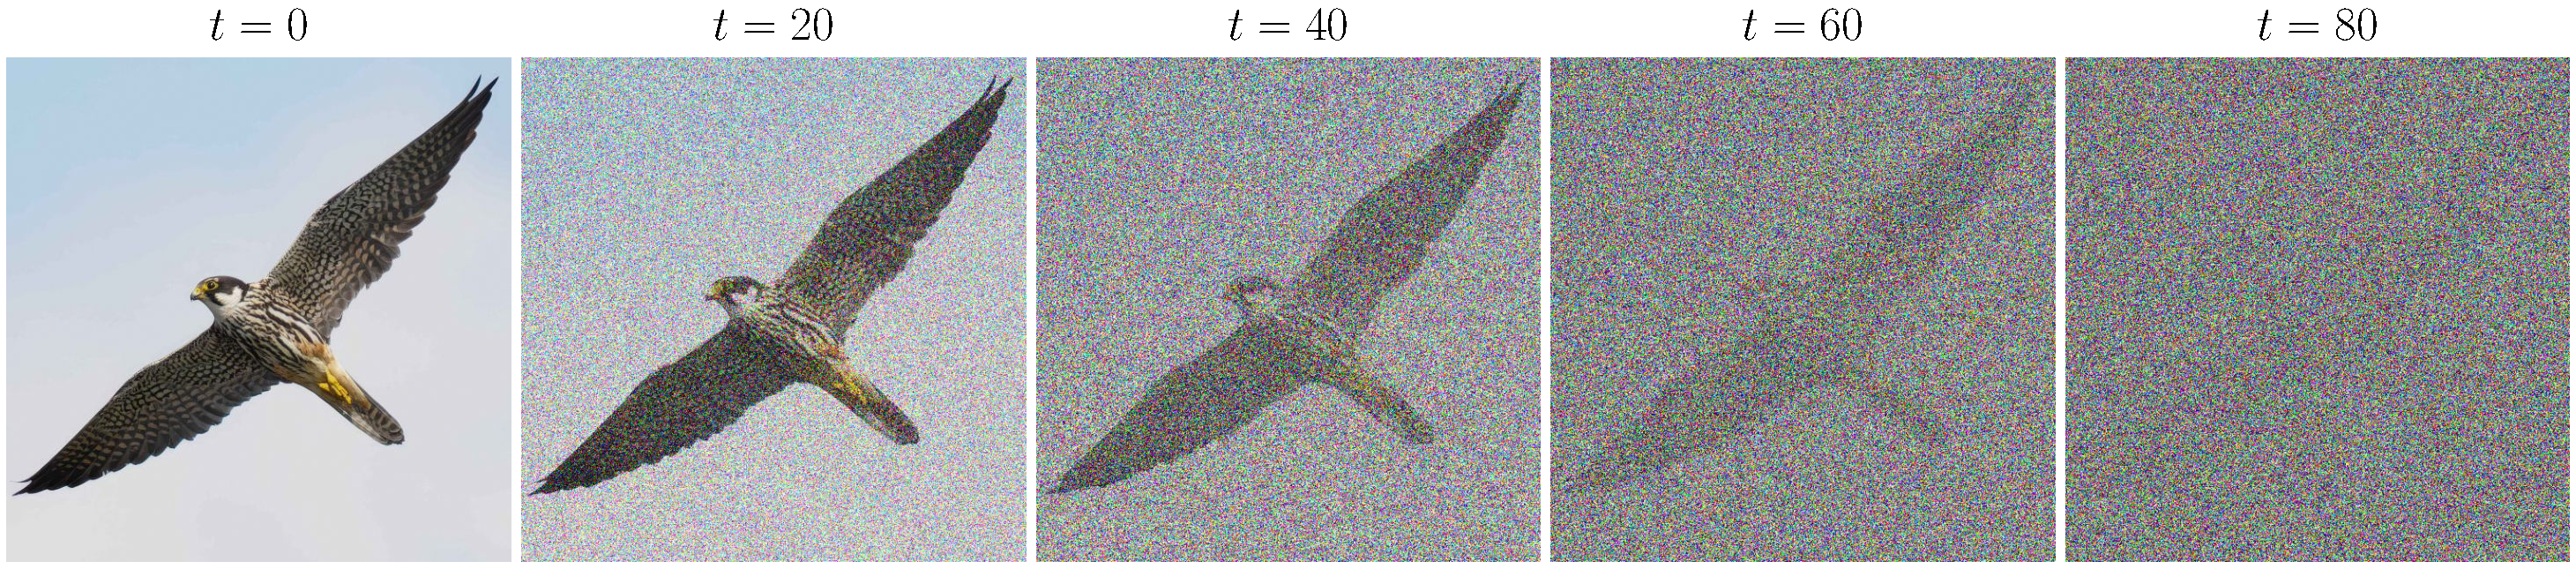
\includegraphics[width=0.85\linewidth]{./Figures/DDPM_Visual.pdf}
		\caption{DDPM\_Visual.pdf}
		\label{Fig_DDPM_Visual}
	\end{figure}
\end{block}
\vspace*{-0.4cm}
\begin{lstlisting}
\begin{figure}[H]
    \centering
    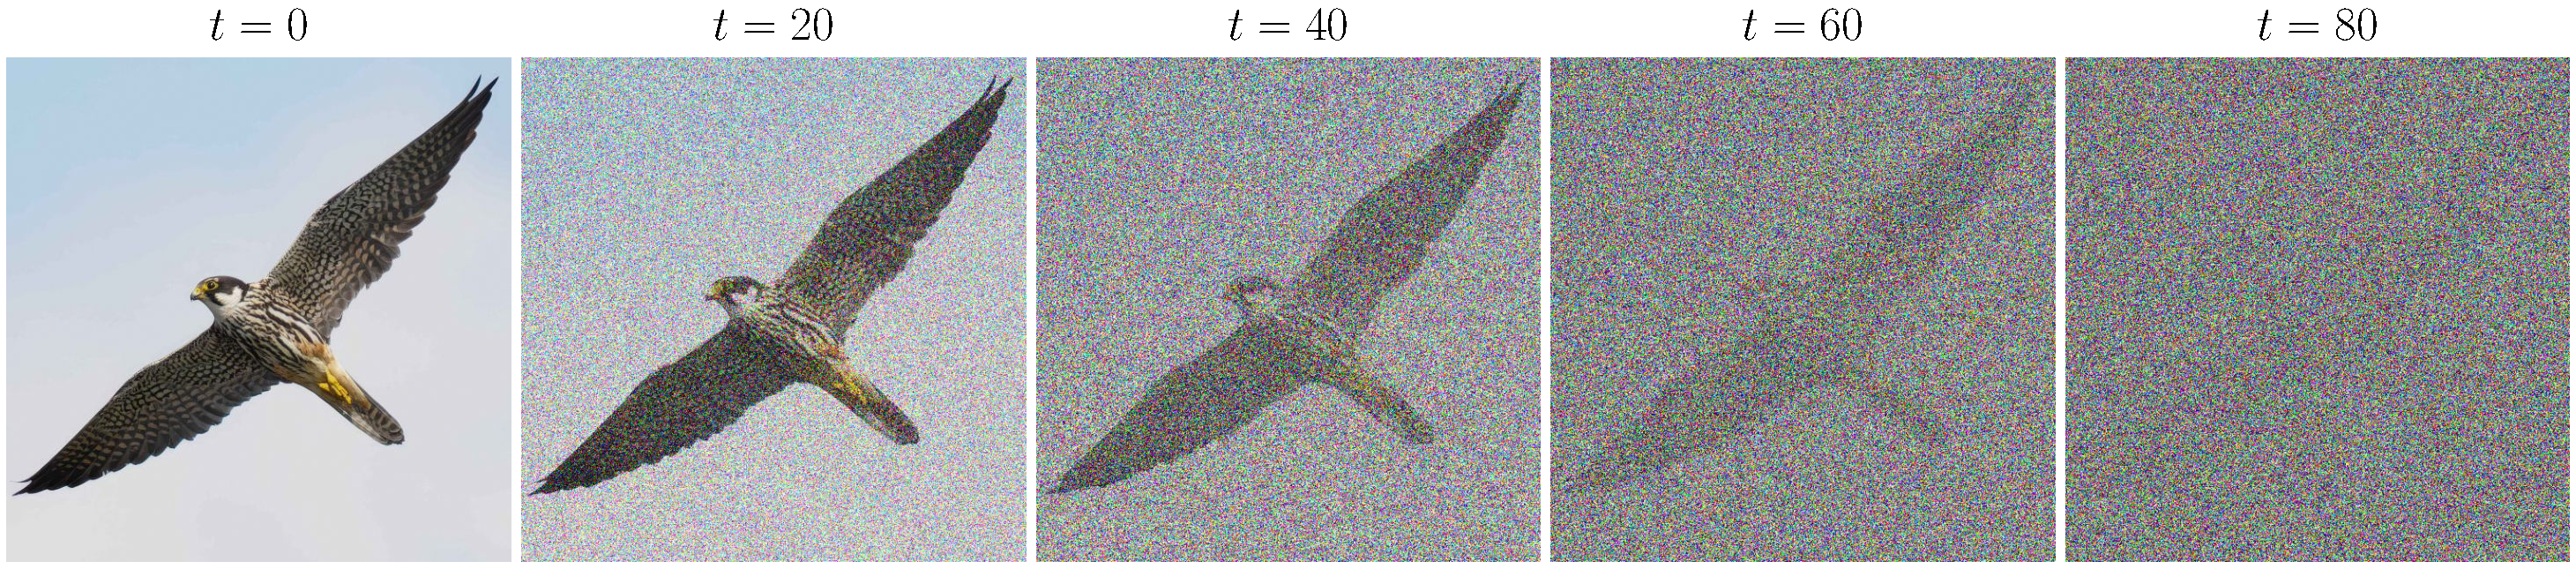
\includegraphics[width=0.3\linewidth]{./Figures/DDPM_Visual.pdf}
    \caption{DDPM\_Visual.pdf}
    \label{Fig_DDPM_Visual}
\end{figure}
\end{lstlisting}

\begin{block}{多子图}
	\begin{figure}[H]
		\centering
		\subfloat[Fig1.png]{
			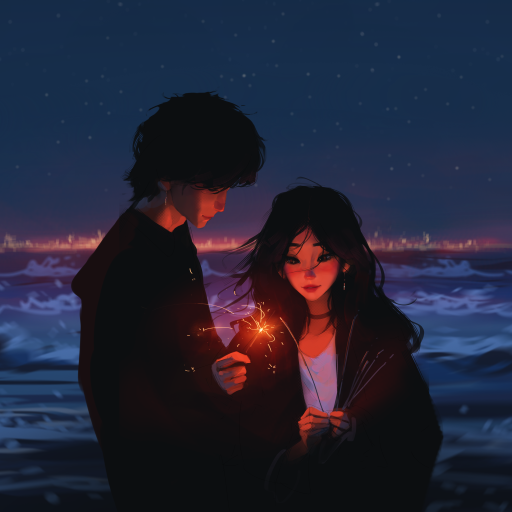
\includegraphics[width=0.18\linewidth]{./Figures/Fig1.png}
		}
		\subfloat[Fig2.png]{
			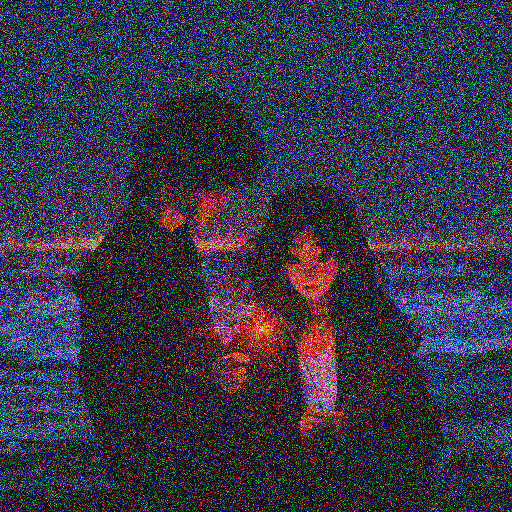
\includegraphics[width=0.18\linewidth]{./Figures/Fig2.png}
		}
		\caption{Fig1.png \& Fig2.png}
		\label{Fig_subfloat}
	\end{figure}
\end{block}
\vspace*{-0.7cm}
\begin{lstlisting}
\begin{figure}[H]
    \centering
    \subfloat[Fig1.png]{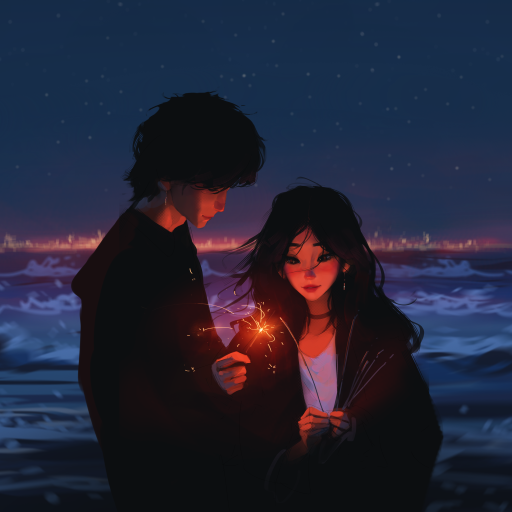
\includegraphics[width=0.2\linewidth]{./Figures/Fig1.png}}
    \subfloat[Fig2.png]{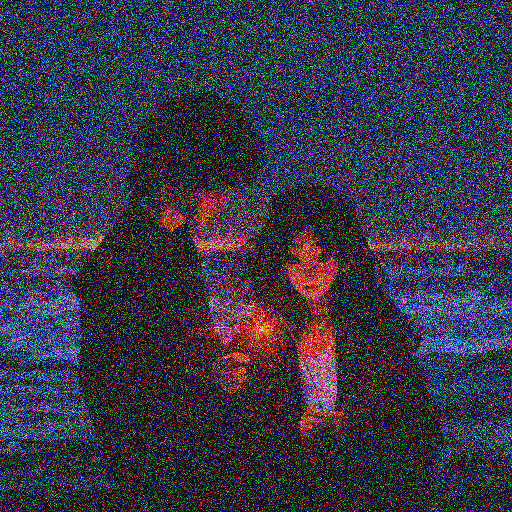
\includegraphics[width=0.2\linewidth]{./Figures/Fig2.png}}
    \caption{Fig1.png \& Fig2.png}
    \label{Fig_subfloat}
\end{figure}
\end{lstlisting}
\end{frame}


\begin{frame}[fragile,allowframebreaks]{表格}
	\begin{block}{表格}
		\begin{table}[H]
			\centering
			\caption{Table Name}
			\label{Table_PSNRandSSIM}
			\footnotesize
			\begin{tabular}{c|c|c||c|c|c}
				\toprule[1.5pt]
				\multirow{2}{*}{\makecell{噪声水平 \\ PSNR / SSIM}} & \multicolumn{2}{c||}{ImageNet32} & \multirow{2}{*}{\makecell{噪声水平 \\ PSNR / SSIM}} & \multicolumn{2}{c}{BSD68} \\
				& 模型名称  & PSNR / SSIM && 模型名称  & PSNR / SSIM \\
				\midrule[0.75pt]\midrule[0.5pt]
				% sigma = 5
				\multirow{5}{*}{\makecell{$\sigma=5$ \\ 34.16 / 0.94}} & BM3D\textsuperscript{\cite{Hunheyu}} & 29.98 / 0.92 & \multirow{5}{*}{\makecell{$\sigma=5$ \\ 39.38 / 0.98}} & BM3D\textsuperscript{\cite{Hunheyu}} & 29.98 / 0.90 \\
				& Shrinkage\textsuperscript{\cite{2014Shrinkage}} & 30.50 / 0.92 && Shrinkage\textsuperscript{\cite{2014Shrinkage}} & 29.11 / 0.90 \\
				& CBDNet\textsuperscript{\cite{2019CBDNet}}          & 37.06 / 0.97 && CBDNet\textsuperscript{\cite{2019CBDNet}}         & 40.07 / 0.98 \\
				& DRANet\textsuperscript{\cite{2024DRANet}}         & 40.55 / 0.99 && DRANet\textsuperscript{\cite{2024DRANet}}          & 40.28 / 0.99 \\
				& \cellcolor[HTML]{EFEFEF}Ours & \cellcolor[HTML]{EFEFEF}38.39 / 0.95 && \cellcolor[HTML]{EFEFEF}Ours & \cellcolor[HTML]{EFEFEF}35.73 / 0.96 \\
				% sigma = 10
				\midrule[0.5pt]\midrule[0.5pt]
				\multirow{5}{*}{\makecell{$\sigma=10$ \\ 28.25 / 0.83}} & BM3D\textsuperscript{\cite{Hunheyu}} & 28.57 / 0.90 & \multirow{5}{*}{\makecell{$\sigma=10$ \\ 33.65 / 0.94}} & BM3D\textsuperscript{\cite{Hunheyu}} & 27.63 / 0.88 \\
				& Shrinkage\textsuperscript{\cite{2014Shrinkage}} & 30.31 / 0.92 && Shrinkage\textsuperscript{\cite{2014Shrinkage}} & 29.03 / 0.90 \\
				& CBDNet\textsuperscript{\cite{2019CBDNet} }         & 32.70 / 0.95 && CBDNet\textsuperscript{\cite{2019CBDNet}}         & 36.46 / 0.97 \\
				& DRANet\textsuperscript{\cite{2024DRANet}}          & 37.05 / 0.98 && DRANet\textsuperscript{\cite{2024DRANet}}         & 36.26 / 0.97 \\
				& \cellcolor[HTML]{EFEFEF}Ours & \cellcolor[HTML]{EFEFEF}36.75 / 0.92 && \cellcolor[HTML]{EFEFEF}Ours & \cellcolor[HTML]{EFEFEF}34.82 / 0.95 \\
				\midrule[0.5pt]\bottomrule[1.5pt]
			\end{tabular}
		\end{table}
	\end{block}
	
	
	\qquad（续表 \ref{Table_PSNRandSSIM}）
	\begin{table}[H]
		\centering
		\footnotesize
		\begin{tabular}{c|c|c||c|c|c}
			\toprule[1.5pt]
			\multirow{2}{*}{\makecell{噪声水平 \\ PSNR / SSIM}} & \multicolumn{2}{c||}{ImageNet32} & \multirow{2}{*}{\makecell{噪声水平 \\ PSNR / SSIM}} & \multicolumn{2}{c}{BSD68} \\
			& 模型名称  & PSNR / SSIM && 模型名称  & PSNR / SSIM \\
			\midrule[0.75pt]\midrule[0.5pt]
			% sigma = 15
			\multirow{5}{*}{\makecell{$\sigma=15$ \\ 24.82 / 0.73}} & BM3D\textsuperscript{\cite{Hunheyu}} & 27.69 / 0.89 & \multirow{5}{*}{\makecell{$\sigma=15$ \\ 30.21 / 0.89}} & BM3D\textsuperscript{\cite{Hunheyu}} & 26.77 / 0.85 \\
			& Shrinkage\textsuperscript{\cite{2014Shrinkage}} & 29.96 / 0.91 && Shrinkage\textsuperscript{\cite{2014Shrinkage}} & 28.88 / 0.89 \\
			& CBDNet\textsuperscript{\cite{2019CBDNet}}          & 29.59 / 0.91 && CBDNet\textsuperscript{\cite{2019CBDNet} }         & 33.78 / 0.96 \\
			& DRANet\textsuperscript{\cite{2024DRANet}}          & 35.08 / 0.97 && DRANet\textsuperscript{\cite{2024DRANet}}         & 34.03 / 0.96 \\
			& \cellcolor[HTML]{EFEFEF}Ours & \cellcolor[HTML]{EFEFEF}34.14 / 0.90 && \cellcolor[HTML]{EFEFEF}Ours & \cellcolor[HTML]{EFEFEF}33.12 / 0.93 \\
			\midrule[0.5pt]\bottomrule[1.5pt]
		\end{tabular}
	\end{table}
	
\begin{lstlisting}
\begin{table}[H]
    \centering
    \caption{Table Name}
    \label{Table_PSNRandSSIM}
    \footnotesize
    \begin{tabular}{表格对齐设置}
        % 表格内容
    \end{tabular}
\end{table}
\end{lstlisting}
\end{frame}


\begin{frame}[fragile,allowframebreaks]{算法流程}
	\begin{center}
		\small
		\begin{minipage}{0.75\linewidth}
			\begin{algorithm}[H]
				% 标题
				\caption{残差噪声扩散模型的推理过程}\label{Resfusion_algorithm_inference}
				\KwIn{
					待恢复退化图像 $\hat{\xb}_0$.
				}
				\KwOut{恢复图像 $\xb_0$.}
				从 $\xb_{T'} \sim \N(\xb_{T'};(1-\sqrt{\bar{\alpha}_{T'}})\hat{\xb}_0,(1-\bar{\alpha}_{T'})\Ib)$ 中抽样 $\xb_{T'}$ \;
				
				\For{$t=T',T'-1,\dots,1$}{
					\eIf{$t>1$}{
						从高斯正态分布 $\zb \sim \N(\zb;\zeros,\Ib)$ 中抽样 $\zb$ \;
					}{
						$\zb=\zeros$ \;
					}
					计算 $\sigma_q(t) = \sqrt{\dfrac{(1-\alpha_t)(1-\bar{\alpha}_{t-1})}{1-\bar{\alpha}_t}}$ \;
					
					计算
					\[
					\xb_{t-1} = \dfrac{1}{\sqrt{\alpha_t}}\left(\xb_t-\dfrac{1-\alpha_t}{\sqrt{1-\bar{\alpha}_t}}res\epsilonb_{\thetab}(\xb_t,\hat{\xb}_{0},t)\right) + \sigma_q(t)\zb
					\]
				}
			\end{algorithm}
		\end{minipage}
	\end{center}
\begin{lstlisting}
\begin{center}
\small
\begin{minipage}{0.75\linewidth}
    \begin{algorithm}[H]
        % 算法内容
    \end{algorithm}
\end{minipage}
\end{center}
\end{lstlisting}
	\vspace*{0.5cm}
	\begin{block}{Tips}
		强烈建议使用 \texttt{minipage} 环境包裹 \texttt{algorithm} 环境，方便控制算法流程的整体宽度。
	\end{block}
\end{frame}


